\chapter{Background}
\label{ch:background}

% material necessary to understand the rest of the thesis

% last section in this chapter is usually related work

\com{
\todo[inline]{When you do your literature study, you should have a nearly complete Chapters 1 and 2.\\
You may also find it convenient to introduce the future work section into your report early – so that you can put things that you think about but decide not to do now into this section.\\
Note that later you can move things between this future work section and what you have done as you may change your mind about what to do now versus what to put off to future work.
}

What does a reader (another x student -- where x is your study line) need to know to understand your report?
What have others already done? (This is the “related work”.) Explain what and
how prior work / prior research will be applied on or used in the degree
project /work (described in this thesis). Explain why and what is not used in
the degree project and give valid reasons for rejecting the work/research.
}


\noindent This chapter presents relevant background research that is needed to understand the current state of the art about mobile robotics, the localisation field, and mapping aspects.

The specific coordinate frame of the wheeled mobile robot adopted for this project, with its kinematics and constraints, are described to present how the robotic lawn mower will be localised, controlled, and constrained.

Afterwards, the focus will be on the localisation topic, starting from an analysis of sensors both already available on the \gls{ALM} and also those useful for positioning.
The focus is about sensors which require no additional infrastructure installation.
Additionally, techniques used to fuse their measurements will be described, shown, and analysed to highlight which technique is the most relevant for this project.

Furthermore, a brief analysis of mapping aspects is presented.
Different mapping algorithms are available and only the most relevant approach for this thesis is discussed.

Finally, theoretical related works are briefly described to highlight their contributions, and a summary of the lessons learned from the literature study is presented.


\section{Mobile Robots}

\noindent Mobile robots are robotics systems which are able to move themselves on the environment they are in.
The mobile robot used in this thesis equips two standard back wheels with differential drive, and two castor wheels on the front which allow free rotation around the wheel axle for multiple direction steering.
An analysis of the coordinate and robot frame is presented, followed by the definition of its kinematic model and by an overview of the constraints involved.

\subsection{Coordinate Frame}

\noindent
The pose of the robot $P_r$ on the global frame frame $G$ is defined by the following \gls{DOF} vector used to localise it in the \gls{2D} environment:
\begin{equation}
    P_r = \begin{bmatrix}x_r&y_r&\theta_r\end{bmatrix}^T
    \label{eq:dof}
\end{equation} where $x_r$, $y_r$, and $\theta_r$ define respectively the translation and rotation of the origin of the robot frame $O_R$ with respect to the origin of the global frame $O_G$, as shown in figure \ref{fig:TikzKine}.
\begin{figure}[!ht]
    \centering
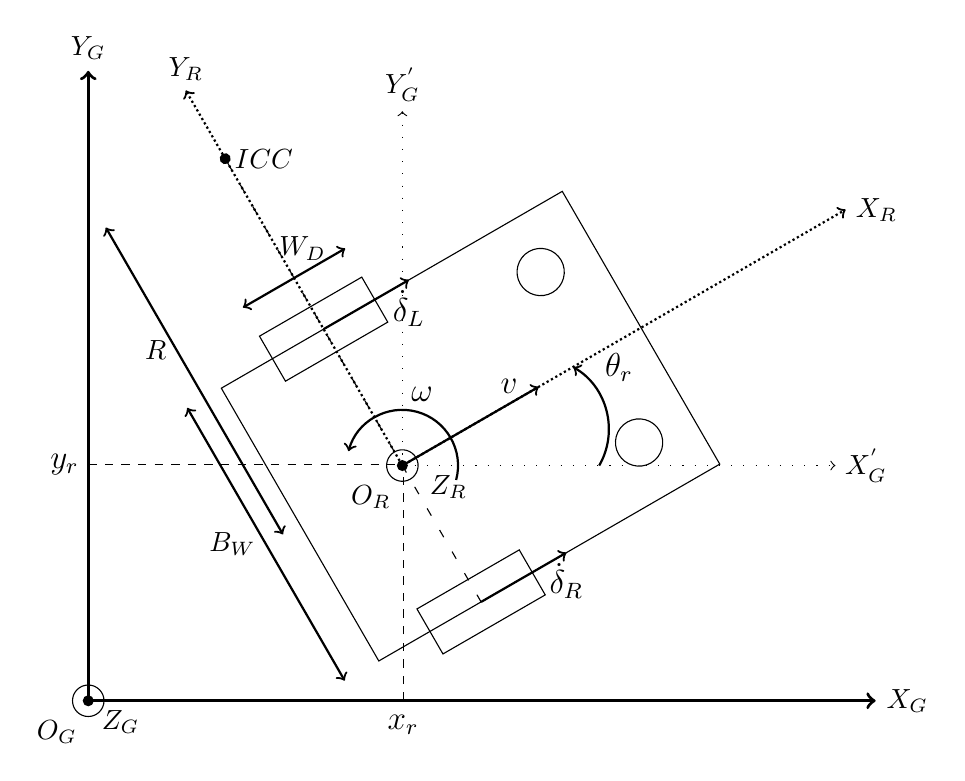
\begin{tikzpicture}
  \draw [<->, very thick]  (0,8) node (yaxis) [above] {$Y_G$} |- (10,0) node (xaxis) [right] {$X_G$};
  \draw (-0.4,-0.4)  node (origin) [] {$O_G$};
  \draw (4,-0.3)  node (x_i) [] {\large$x_r$};
  \draw (-0.3,3)  node (y_i) [] {\large$y_r$};
  \draw[black] (0, 0) circle (0.2) node (z) [below] {~~$~~~~~Z_G$};
  \fill[black]  (0,0)   circle (2pt);
  \draw[ dashed] (4,0) -- (4,3);
  \draw[ dashed] (0,3) -- (4,3);
  \begin{scope}[xshift=113.5, yshift=85]
        \fill[black]  (0,0)   circle (2pt);
          \draw [<->, loosely dotted]  (0,4.5) node (yaxisG) [above] {$Y_G^{'}$} |- (5.5,0) node (xaxisG) [right] {$X_G^{'}$};
          \draw (-0.4,-0.4)  node (origin_r) [] {$O_R$};
          \draw[->, thick]  (2.5,0) to[out=60,in=-30, distance=0.5cm] (2.17,1.25) node (theta) [below, right] {\large$~~\theta_r$} ;
      \begin{scope}[rotate=30]
          \draw [<->, densely dotted, thick]  (0,5.5) node (yaxis_r) [above] {$Y_R$}
                |- (6.5,0) node (xaxis_r) [right] {$X_R$};
          \draw[->, thick]  (0.5,-0.5) to[out=45,in=-45] (0.5,0.5)  node (omega) [above] {\large$~\omega$} to[out=135,in=45] (-0.5,0.5);
          \draw [->, thick] (0,0) -- (2,0) node (vel) [above, left] {\large$v$~~};
          \draw [->, thick] (0,2) -- (1.25,2) node (v_L) [below] {\large$\dot \delta _L$};
          \draw [->, thick] (0,-2) -- (1.25,-2) node (v_R) [below] {\large$\dot \delta _R$};
          \draw[<->, thick]  (-2,-2) -- (-2,2) node (base) [pos=0.5, below, left] {$~B_W$} ;
          \draw[<->, thick]  (-0.75,2.75) -- (0.75,2.75) node (diameter) [above, left] {$W_D$~~} ;
          \draw[<->, thick]  (-1.75,0) -- (-1.75,4.5) node (curvature) [pos=0.6, below, left] {$R$} ;
          \draw[-, loosely dashed]  (0,-2) -- (0,4.5) ;
            \fill[black]  (0,4.5)   circle (2pt);
            \draw (0,4.5)  node (ICC) [above, right] {$ICC$};
        \draw[black]  (-0.75,-2.33) rectangle (0.75,-1.67);
        \draw[black]  (-0.75,2.33) rectangle (0.75,1.67);
        \draw[black] (-1.5,-2) rectangle (3.5,2);
        \draw[black] (2.75, 1.25) circle (0.3);
        \draw[black] (2.75, -1.25) circle (0.3);
        \draw[black] (0, 0) circle (0.2) node (z) [below] {~~$~~~~~~~~Z_R$};
      \end{scope}
  \end{scope}
\end{tikzpicture}
  \caption{Kinematic model of a differential drive mobile robot.}
  \label{fig:TikzKine}
\end{figure}

The rotational and translational relations between frames is provided by the transformation matrix $T^G_R$, used to transform a point of the robot frame $P_R$ to a point of the global frame $P_G$, as defined in the following equation:

\begin{align}
P_{G} = T^G_R \cdot O_{R} && \text{with } && T^G_R =
\begin{bmatrix}
cos(\theta_r) & -sin(\theta_r) & x_r \\
sin(\theta_r) & cos(\theta_r) & y_r \\
0 & 0 & 1 \\
\end{bmatrix}
\label{eq:transfPoint}
\end{align}

For the scope of this thesis, just the kinematics have been considered as other aspects, such as torque, friction, physical implications, and in general the dynamics of the systems, are not relevant to be analysed for the scope of this thesis.

\subsection{Kinematic Analysis}
\label{ssec:kin_a}
\noindent
The \gls{ALM} consists of two drive back wheels mounted along the same axis.
Each wheel is actuated independently either in forward or backward rotation.
By varying the velocity of each wheel, the robot rotates around a \gls{ICC}~\cite{ICC}, $ICC$ in figure \ref{fig:TikzKine}, defined directly by its distance from the robot origin, $R$, varying the wheel velocities, $\dot \delta_L$ and $\dot \delta_R$, as in equation \eqref{eq:R}:
\begin{equation}
    R = \cfrac{\dot \delta_R + \dot \delta_L}{\dot \delta_R - \dot \delta_L} \cdot \cfrac{B_W}{2}
    \label{eq:R}
\end{equation}
where $B_W$ defines the base width of the \gls{ALM} as distance between wheels.
Using this approach it is possible to vary the trajectory that the robot follows varying the wheels' velocities, i.e. in case the wheels' velocities are equal, $R$ will result to be infinite and the robot will not rotate, following a straight trajectory.
Some constraints about the possible trajectories are explained in section \ref{sec:constraints}.

The rate of rotation about $ICC$ is the same as the velocity of rotation around the robot frame origin $O_R$, defined by the time derivation of its orientation $\theta_r$. This angular velocity, $\omega$, is used to control the trajectory of the robot and it is defined as in equation \eqref{eq:omega}.
\begin{equation}
    \omega = \cfrac{\partial{\theta_r}}{\partial{t}} = \cfrac{\dot \delta_R - \dot \delta_L}{B_W}
    \label{eq:omega}
\end{equation}

The differential drive mobile robot is controlled directly through the desired linear velocity $v$ along the $X_R$ axis of the robot, and the desired angular velocity $\omega$ around the $Z_R$ axis.
The angular velocity is defined above in equation \eqref{eq:omega} and the linear velocity is defined as a transformation of the angular velocity, or of the wheel velocities, as in equation \eqref{eq:vel}.
\begin{equation}
    v = \omega \cdot R = \cfrac{\dot \delta_R + \dot \delta_L}{2}
    \label{eq:vel}
\end{equation}

As the differential mobile robot is propelled by two separate motors mounted on the back wheels, its movements are defined by the wheel actuators and thus the desired control velocities need to be transformed into the proper wheels' velocities using the following equations \eqref{eq:wheel_vel}.
\begin{align}
    \dot \delta _L  & =\omega \cdot ( R - \frac{B_W}{2} ) &
    \dot \delta _R  & = \omega \cdot ( R + \frac{B_W}{2})
    \label{eq:wheel_vel}
\end{align}


\subsection{Constraints}
\label{sec:constraints}

\noindent
This differential drive system is not able to freely move along the \gls{2D} environment, as the degrees of freedom, defined in \eqref{eq:dof}, are less than degrees of mobility, given by the control velocities, $v$ and $\omega$.
The system is thus called non-holonomic and a non-holonomic constraint has to be defined.
The standard wheels used by the differential mobile robot are subject to such non-holonomic rolling constraint, which limits the sideways sliding by imposing that the wheel spins purely along the direction of the wheel.
For example, to perform the rolling motion along the $Y_R$ axis, the robot will have to vary the velocity of each wheel to rotate around its origin to align itself along that initial direction before moving forward.
Non-holonomic constraints do not allow for integration of the differential equations to retrieve the final pose, since the displacements of each wheel are not sufficient to determine it.
This forces the position and orientation to be estimated using integration of wheels velocities rather than their position displacements.
However, with a sufficient sampling rate, an integrable approach can be used to estimate its pose, but the usage of incremental displacements provided by integration of wheels' velocity measurements will inevitably accumulate errors over time.

\com{
\section{Localisation}
\noindent As this is the main topic of this project, an extensive analysis of this field will be performed.
Understanding the current state-of-the-art of localisation and its possible improvement is required.

Firstly, the available sensors that could be installed directly on the mobile robot, that do not require additional installation of infrastructures, and that can be used to improve localisation are described below.

Afterwards, different techniques available to fuse their heterogeneous measurements are described in their performances.
}

\section{Sensors}



\noindent For a robot to localise itself, it needs to perceive its surroundings and to do so it relies on its sensors' measurements.
These sensors perceive and interpret different recorded phenomena based on their characteristics, and they can be divided in three main different types.
\textit{Interoceptive sensors} focus on internal data measured directly by the mobile robot. They output engineering quantities which are used to estimate how the system is behaving internally, e.g. wheel encoders.
\textit{Proprioceptive sensors} measure robotic's interaction with the environment. They provide a value of how the movements of the mobile robot are perceived with respect to the outside, e.g. accelerometers, or gyroscopes.
\textit{Exteroceptive sensors} provide measures related directly to their perception of the external environment. The information they measure are related to phenomena happening at the environments around the mobile robot, e.g. magnetometers, \glspl{GNSS}, or cameras.

As they measure different aspects, they perform differently.
They provide advantages and disadvantages which can be combined in an intelligent manner to exploit their capabilities and limit their inaccuracies.

The available sensors that could be installed directly on the mobile robot, that do not require additional installation of infrastructures, and that can be used to improve localisation are described below.

\subsection{Wheel Encoder}

\noindent This interoceptive sensor detects the number of revolutions of the wheels, and they can be used to estimate their velocity~\cite{encoder}. An example of the optical wheel encoder is given in figure \ref{fig:encoder}.
\begin{figure}[!ht]
  \begin{center}
    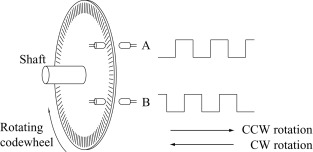
\includegraphics[width=0.65\textwidth]{Images/2-Background/Enc.jpg}
  \end{center}
  \caption{Optical wheel encoder and resulting encoded signal~\cite{wheelEncoder}.}
  \label{fig:encoder}
\end{figure}

This sensor relies on a rotary encoding disk attached to the wheel axis on the end of the motor that estimates the relative angle change of the wheel.
Rotary encoders can be of different kinds based on which phenomenon they observe: mechanical, optical, or magnetic.
Incremental encoders estimate the relative rotation of the wheels by detecting the number of pulses, defined by step signals A and B in Figure \ref{fig:encoder}, within certain time period using the internal clock of the embedded computer.

Wheel encoders are often chosen for \gls{DR}, i.e. the estimation of the pose using previous estimate and velocity, because of their fast measurement rate and their inexpensiveness.
Related to the field of sensor fusion, these are key aspects to consider, as their employment is effective if combined with other sensors. They will be able to provide fast accurate velocity measures which could be used to compute a short-term accurate \gls{DR}.

The estimate derived from the wheel encoders is called \gls{WO} and it is subjects to errors and their accumulation.
Some non-systematic errors related to these sensors are the miscalculations caused by slippage, uneven terrain, and other environmental issues which include wheels temperature and pressure of their tires.
In order to improve its \gls{DR} estimates, other sensors' measurements can be combined with its velocity estimates to get rid of the integration error accumulation on its position calculations.


\subsection{Inertial Measurement Unit}

\noindent An \gls{IMU} is an inertial sensor which is used to detect multiple phenomena and which measurements are relative to the inertial frame of platform they are attached to.
They have both proprioceptive and exteroceptive characteristics as they contain both accelerometers, gyroscopes, and magnetometers.
These sensors are placed in each orthogonal axis to provide measurements for each degree of freedom in free space, as shown in figure \ref{fig:imu}.
Recent \glspl{IMU} are developed on \glspl{MEMS} which are inexpensive and provide measurements with a high sampling rate.
\begin{figure}[!ht]
  \begin{center}
    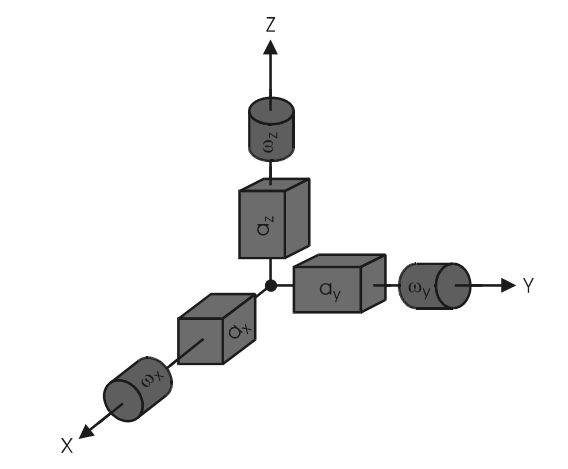
\includegraphics[width=0.5\textwidth]{Images/2-Background/IMU-2021-04-23 14-13-19.png}
  \end{center}
  \caption{Structure of accelerometers and gyroscopes of an \Gls{IMU}~\cite{inertial}.}
  \label{fig:imu}
\end{figure}

Accelerometers measure the linear accelerations, gyroscopes output the rotational velocities, and magnetometers detect the earth magnetic field.
Knowing these measures, the position and orientation can be estimated by integrating those signal over time with a \gls{DR} approach.
Their measurement are prone to deterministic errors, such as repeatable terms and temperature induced variations, and to stochastic errors as switch-on to switch-on variations, and in-run variations~\cite{magnusson_improving_2012}.
Deterministic errors can be compensated for through prediction and calibration, while stochastic ones are more difficult to model because of their noise and randomness.
Accelerometers and Gyroscopes are sensors that need no external support, and they are not conditioned by external conditions or disturbances as they measure proprioceptive characteristics.
Magnetometers instead might be conditioned by external disturbances as the magnetic field can be disturbed by multiple external factors, as any electronic device has a magnetic influence.

They provide accurate results over a short time span, but the integration of noisy results implies an accumulation of these errors over time. This phenomenon then leads to a diverging drift effect, if not corrected by other sensor measurements.


\subsection{Global Navigation Satellite System}

\noindent \glspl{GNSS} are exteroceptive systems based on signals received from satellites orbiting earth.
A \gls{GNSS} receiver uses trilateration to estimate its position on the globe using time of flight of the signals sent by some satellites.
The signals sent by satellites are composed by their trajectory, called ephemeris, along with their internal reference timestamp, and they are used to estimate their range as shown in figure \ref{fig:gps}.
\begin{figure}[!ht]
  \begin{center}
    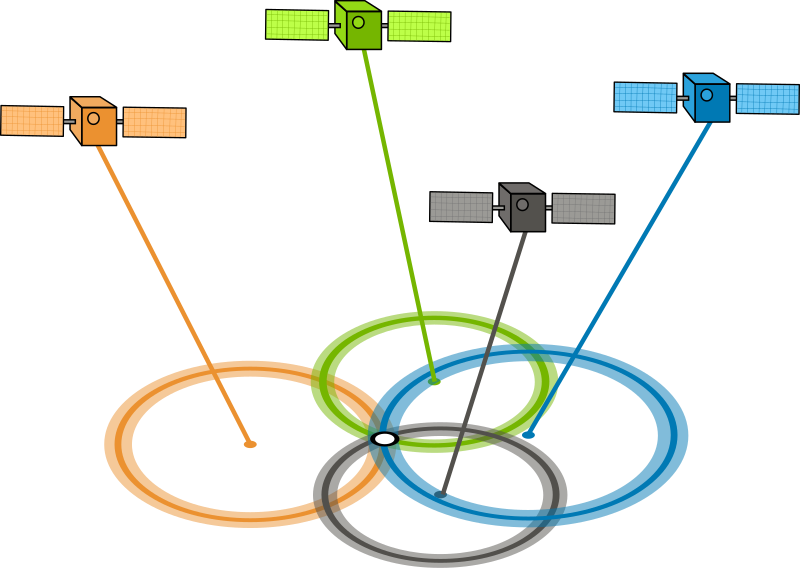
\includegraphics[width=0.5\textwidth]{Images/2-Background/GPS.png}
  \end{center}
  \caption{Trilateration for \Gls{GNSS}, including range error bars.}
  \label{fig:gps}
\end{figure}

The configuration of perceived satellites contributes to their accuracy, as close position of several satellites implies that their range will be close, and their signals will not be effective.
A more spread configuration of satellites' range reduces the \gls{DOP}, which compares the position error to the satellite range error.
Other source of errors are related to conditions which directly affect the time of flight of the signal, such as the presence of ionospheric and tropospheric delays, and the positioning in dense and noisy environments.
The performance of these sensors is thus highly dependent on their environment.

For the \gls{GNSS} receiver to estimate its position, it need to acquire measurements from at least four satellites.
Three satellites signals are used to triangulate the \gls{3D} position and the fourth is used for the synchronization of the clocks, essential to compensate eventual time differences between the receiver and the satellites.
In case the perceived satellites are less then required, the receiver will have a system outage, not being able to estimate its position and velocity.
As there exist multiple \gls{GNSS} systems developed by distinct entities with different original purposes and number of satellites, some \gls{GNSS} sensors are able to receive signals from different systems to improve their satellite coverage and their precision.
With a higher number of perceived satellite signals, the receiver is able to use redundant information to increase its robustness to external disturbances and improve its position measurement accuracy.

The sampling rate of \gls{GNSS} receivers is usually around one estimate per second, thus it is generally too slow to estimate the position for vehicles.


\subsection{Camera}

\noindent A camera sensor is an exteroceptive sensors, usually composed of lenses and light sensors, which gathers the \gls{RGB} information from the environment.
Recent camera models are able to estimate stereopsis data, i.e. depth measurements can be estimated.
A typology of such a sensor is the structured-light camera. It projects an infrared mesh pattern in the environment and then uses stereo cameras to perceive this pattern and it triangulates the depth based on the density of the projected points.
Multiple factors can lower this sensor performances, such as excessive lightning conditions and reflecting materials which modify the infrared pattern.

These sensors can be used with a process called \gls{VO} to estimate the incremental movement of the camera, and the robot at which they are attached, by the changes detected in adjacent images with a \gls{F2F} method.
The \gls{VO} algorithm detects the position of some specific features and then matches those landmarks in two consecutive images.
By knowing their relative pose changes and the configuration of the camera, it is possible to estimate the corresponding camera movement
The performances of this technique relies on the identification of landmarks, the more visible and variant landmarks are detectable, the more the pose estimation will be accurate.
Those features are computed using different descriptors, e.g. \gls{SIFT}, \gls{SURF}, and \gls{ORB}.
The matching phase is guided by an initial estimate of the camera movement which projects previously found features to search just along that projection.
The landmarks are matched after passing a consistency test and those displacements are triangulated to estimate the camera pose through a bundle adjustment step~\cite{robustFusion}, as shown in figure \ref{fig:camera}.

\begin{figure}[!ht]
  \begin{center}
    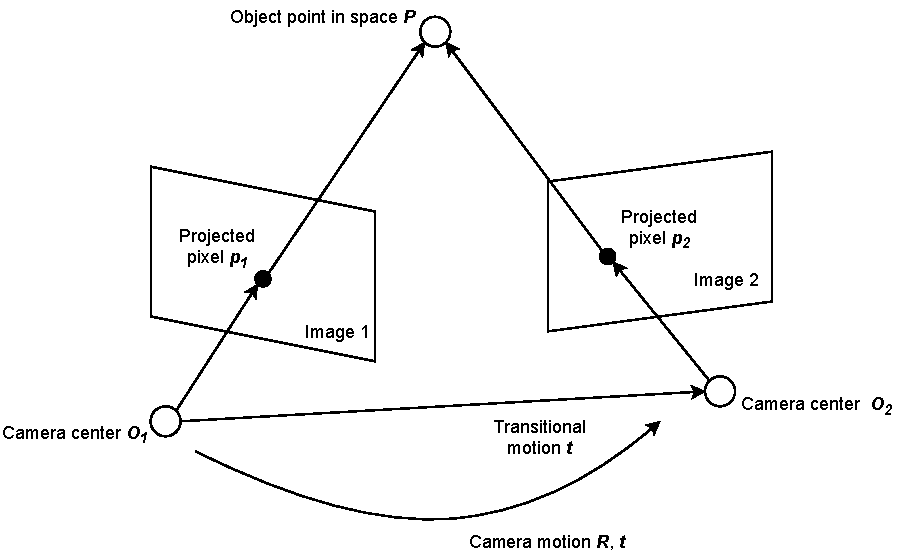
\includegraphics[width=0.65\textwidth]{Images/2-Background/VO.pdf}
  \end{center}
  \caption{Motion estimation via \gls{F2F} methodology~\cite{camera}~\cite{cameraa}.}
  \label{fig:camera}
\end{figure}

Instead of using a more complex \gls{SLAM} algorithm where all the position of the landmarks are also used to estimate a map of the environment, in the \gls{VO} case the landmarks are used just for the displacement analysis, not storing the landmark positions over time.
Using this approach, just the previous state will be saved to estimate the offset, this results in faster computations, and thus an higher sampling frame rate.
This is a key aspect, since we aim to use this approach in an embedded system for a real-time application. However, the estimates in velocity between frames derived from the \gls{VO} is used to compute a \gls{DR} localisation and it is subjects to drift.

%Different techniques are available to compute the features and derive the estimations from the frames, with different implementations such as ORB-SLAM2 and RTABMap, where each of them provide odometry measure with different settings. Some examples are briefly shown in~\cite{Fast and robust visual odometry with a low-cost IMU in dynamic environments Erliang Yao, Hexin Zhang and Haitao Song}

Given the still relatively low frequency of the \gls{VO}, high linear and angular velocities will render the \gls{VO} estimation inaccurate, as it will be more difficult for the system to match identified landmarks when their displacement is bigger.



\section{Sensor Fusion}

\noindent
In the field of localisation for mobile robots, sensor fusion is employed to combine redundant and complementary measurements from heterogeneous sensors to gain a more precise understanding of the pose in the environment.
An issued related to the sensor fusion problem is the determination of the best configuration to combine the measurements of multiple different sensors.
The objective of sensor fusion is to merge the knowledge acquired by these sensors to improve the position estimate with a more accurate solution with respect to any of the individual data sources trying to mitigate their drawbacks and to maintain their best provided features~\cite{mitchell_multi-sensor_2007}.

Sensor fusion could be characterised based on their competitive, complementary, and cooperative approaches~\cite{1199023}.
Competitive fusion happens when the same attribute is estimated by different sensors to increase the system's robustness.
Complementary fusion is related to the merging the observations of different phenomena to describe the complete system's behaviour.
Cooperative fusion combines measures from different sources to provide information that will not be obtained by a single sensor.

Sensor fusion is related to independent measures and it can be differentiate into multiple categories: sensors, attributes, domains, and time~\cite{weckenmann_multisensor_2009}.
The fusion across different sensors involves merging the same measured phenomenon from different devices to increase the robustness of the measured data, in a competitive approach.
Fusion among different attributes is focused on sensors which estimates different but connected measures which might be related by kinematics or dynamics aspects, improving their precision in a complementary way.
Different domains are fused when sensors measure the same attribute with a different range or frame, improving their performances when one of these sensors reaches its limits, through a cooperative procedure.
Sensor fusion across time merges measure arrived at different times with increasing reliability to increase the evolution of the estimates.

The most common approach to sensor fusion is through the usage of statistical methods, where the uncertainties of the sensors are described by probabilistic models~\cite{gustafsson_statistical_2010}.
This section will describe the basics of some statistical filters used for sensor fusion purposes.
The \gls{KF} will be detailed as it is the most basic among them, followed by an analysis of its non-linear correspondent, the \gls{EKF}. 
These different techniques available to fuse their heterogeneous measurements are described in their performances.

\subsection{Kalman Filter}

\noindent The \gls{KF} was first developed by R.E. Kalman and published in~\cite{kalman} as a Bayesian estimator used in linear Gaussian systems.
The usage of \gls{KF} is ideal for real time, embedded, and sensor fusion systems as it can estimate dynamic systems disturbed by sensor noise with high performances.
It does not require to store in memory the history of all the previous states and they are computationally efficient.

It uses a recursive probabilistic approach to efficiently filter discrete estimates of the states of a process and its estimated uncertainty, and then through new measurements it corrects its state and decreases its uncertainty with the goal of minimising the \gls{LMSE}.
To reach an optimal estimation, at each iteration it performs a weighted sum of its current estimate using the prior estimate and new measurements, and weighting them based on their relative uncertainty.
The \gls{KF} holds information about its estimate and uncertainty through, respectively, the state vector $\mathbf{X}_t$, which contains the states and descriptions of the system, and the state covariance matrix $P_t$,  which holds information about the variance between those states as statistical error indicator.
It is structured as continuous cycle of its iterative process, composed of a prediction and correction phase.

The prediction phase estimates the next state based on the previous one, eventual control inputs, and adding Gaussian white noise to account for uncertainties in the prediction estimate.
\com{
We proceed under the Markovian assumption that p(xk)=∫∞−∞p(xk|xk−1)p(xk−1)dxk−1, meaning that the distribution over the state of an object at time k can be predicted entirely from its state at previous time k−1. (\url{https://stonesoup.readthedocs.io/en/latest/auto_tutorials/01_KalmanFilterTutorial.html#prediction})
}
First of all, the \gls{KF} computes the prediction of the current estimate $\hat{\mathbf{X}}_{t+1}$ using its previous estimate $\mathbf{X}_t $, the transition matrix $A$, and eventual inputs $B \cdot \mathbf{u}_t$, as in equation \eqref{eq:pred-state}.%, and the state noise vector $\boldsymbol \eta_t$:
\begin{align}
\hat{\mathbf{X}}_{t+1} & = A \cdot \mathbf{X}_t + B \cdot \mathbf{u}_t % + \boldsymbol \eta_t
  \label{eq:pred-state}
\end{align}
where the state, being a Gaussian random variable, can be described with its mean and covariance as $\mathbf{X}_{t} \sim \mathcal{N}\left(\mathbf{X}_{t},P_{t}\right)$.%, and its Gaussian noise as $\boldsymbol \eta_t \sim \mathcal{N}\left(0, Q\right)$.
Then, the prediction of the current state covariance $\hat{P}_{t+1}$ is computed using the previous state covariance $P_t$, the transition matrix $A$, and the state noise covariance $Q$, as in equation \eqref{eq:pred-cov-p}.
    \begin{align}
    	\label{eq:pred-cov-p}
        \hat{P}_{t+1} & = A \cdot P_t \cdot A^T + Q
    \end{align}


After a noisy measurement $\mathbf{Z}_{t+1}$ has been obtained, the correction phase corrects the prediction based on the uncertainty of both the prediction and the measurement to improve the estimation of the state.
As first step in the correction, the prediction of the estimated measurements, $\hat{\mathbf{z}}_{t+1}$, is obtained using the measurements matrix $H$, as in equation \eqref{eq:pred-measure}.
    \begin{align}
    \hat{\mathbf{Z}}_{t+1} & = H \cdot \hat{\mathbf{X}}_{t+1}
    \label{eq:pred-measure}
    \end{align}
Then, the innovation vector, $\mathbf{Y}_{t+1}$, is computed as the difference between the estimated measurements and the actual measurements $\mathbf{Z}_{t+1}$:
    \begin{align}
    \mathbf{Y}_{t+1} & = \mathbf{Z}_{t+1} - \hat{\mathbf{Z}}_{t+1}
    \end{align}
Its related innovation covariance, $S$, is given by the following formula, where $R$ is the measurements process noise:
    \begin{align}
    S & = H \cdot \hat{P}_{t+1} \cdot H^T + R
    \end{align}
The Kalman gain, $K$, is then computed to improve the estimate as a relation between state covariance and innovation covariance, related to the measures obtained as follows:
    \begin{align}
    K & = \hat{P}_{t+1} \cdot H^T \cdot S^{-1}
    \end{align}
The corrected state, $\mathbf{X}_{t+1}$, is then obtained using the predicted state and the innovation vector weighted by the innovation covariance:
    \begin{align}
    \mathbf{X}_{t+1} & = \hat{\mathbf{X}}_{t+1} + K \cdot \mathbf{Y}_{t+1}
    \end{align}
Finally, the corrected covariance matrix of the state, $P_{t+1}$, is obtained by equation \eqref{eq:standard-corr-cov}.
    \begin{align}
    	\label{eq:standard-corr-cov}
    P_{t+1} & = (I - K \cdot H) \cdot \hat{P}_{t+1}
    \end{align}

After this, the loop of equations restarts from the prediction phase by updating the time pedix from $t+1$ to $t$, following the structure defined in figure \ref{pic:kalm}.

\tikzstyle{block} = [draw, rectangle, minimum width=6em, align=center,fill=gray!5]
\tikzstyle{arrow} = [-latex, very thick]
\newcommand*{\tran}{\top}

\begin{figure}[!ht]
\centering
\begin{tikzpicture}[auto, node distance=2cm,>=latex']
    \setlength{\abovedisplayskip}{0pt}

    % Place the blocks
    \node[text width=1cm, rounded corners=3pt, block,
          label={[above,align=center]{Initial State}}] at (-2, 0) (initial)
          {\begin{align*}\mathbf{X}_0 \\ P_0\end{align*}};
    \node at (0.0, 0.0) (sum) {};
    \node[block, text width=6cm,
          label={[above,align=center]{Prediction}}] at (4, 0) (prediction)
          {\begin{align*}
        \hat{\mathbf{X}}_{t+1} & = A \cdot \mathbf{X}_t + B \cdot \mathbf{u}_t \\ % + \boldsymbol \eta_t\\
        \hat{P}_{t+1} & = A \cdot P_t \cdot A^T + Q
           \end{align*}};
    \node [block, right of=prediction,
            node distance=3cm, text width=2.4cm,
            label=above right:{New}, label=below right:{Measure}] at (5, -1.33) (iterUpdate)
            {$\mathbf{Z}_{t+1}$};
    \node [block, left of=prediction,
            node distance=3cm, text width=2.4cm,
            label=left:{Next step}] at (2.8, -1.33) (iterChange)
            {$$t+1 \rightarrow t $$ };
    \node [block, text width=6cm,
           label={[above,align=center]{Correction}}] at (4, -4) (innovation)
           {\begin{align*}
    \hat{\mathbf{Z}}_{t+1} & = H \cdot \hat{\mathbf{X}}_{t+1}\\
    \mathbf{Y}_{t+1} & = \mathbf{Z}_{t+1} - \hat{\mathbf{Z}}_{t+1}\\
    S & = H \cdot \hat{P}_{t+1} \cdot H^T + R\\
    K & = \hat{P}_{t+1} \cdot H^T \cdot S^{-1} \\
    \mathbf{X}_{t+1} & = \hat{\mathbf{X}}_{t+1} + K \cdot \mathbf{Y}_{t+1}\\
    P_{t+1} & = (I - K \cdot H) \cdot \hat{P}_{t+1}
            \end{align*}};

    % Connect the nodes
    \draw [arrow] (initial) -- (prediction);
    \draw [arrow] (prediction.east) -| (iterUpdate.north);
    \draw [arrow] (iterUpdate) |- (innovation);
    \draw [arrow] (innovation.west) -|  (iterChange);
    \draw [arrow] (iterChange) |-  (prediction);

\end{tikzpicture}

  \caption{Structure of the Kalman Filter}
  \label{pic:kalm}
\end{figure}

Its many components can are structured in multiple ways.
The initial state $\mathbf{x}_{0}$ can be defined either by zeros or starting estimates or according to the first measurements.
The starting uncertainty of the filter $P_0$ can be initialized with the identity matrix or directly with the state noise covariance. In both cases, the filter will need some steps before converging to more stable estimates of state and covariance.
The state noise covariance $Q$ is harder to determine, as the transition equations would need to specify maximum bounds to define its components.
The measurement noise covariance $R$ is composed by the variances of its components and they are usually estimated through calibration.
If the state and measurement noises change over time, their matrices $Q$ and $R$ needs to be updated as the filter runs, as it is their relative ratio which determines how the Kalman gain $K$ is defined to improve the estimates. In this case, the \gls{KF} is defined as Adaptive~\cite{adaptive}~\cite{1099422}.


An numerical evaluation improvement over the standard \gls{KF} is directly given by changing the state covariance correction step using the Joseph’s form~\cite{schmidt_analysis_2010}, defined by:
\begin{equation}
    P_{t+1} = (I - K \cdot H) \cdot \hat{P}_{t+1} \cdot (I - K \cdot H)^T + K \cdot R \cdot K^T
\end{equation}
As the standard state covariance correction in Equation \eqref{eq:standard-corr-cov} is composed by subtraction, which can result in a loss in symmetry and positive-definiteness due to rounding errors in a finite word length computer, the Joseph’s form state covariance correction maintains positive and non-zero eigenvalues in $P_t$ through a more computationally demanding equation~\cite{BarShalom2001EstimationWA}.

For the filter to be considered an optimal estimator, it needs to exploit the properties of the Gaussian uncertainties, meaning that the disturbances in both the process and measurements need to be composed by Gaussian white noise.
Moreover, the prediction and correction phases are formulated with the assumptions that the state $\mathbf{X}_t$ is markovian, i.e. that is evolution depends solely on its previous value, and that the measurement $\mathbf{Z}_{t+1}$ only depends on the state $\mathbf{X}_{t+1}$, and not on previous measurements.
When these assumptions are validated, the \gls{KF} is proven to be the best linear estimator possible.
However, it can be used with reasonable results even if the assumptions are not true, i.e. when the noise is not Gaussian and the system is non linear, but in those cases other filters will perform better and must be preferred, such as the ones described below.
In any case, as the \gls{KF} needs multiple iterations to stabilise, if its state is observable, the performance of the algorithm should not account for the first steps.

\subsection{Extended Kalman Filter}

\noindent The \gls{EKF} is an extension of the \gls{KF} used to estimate non linear systems, where equations \eqref{eq:pred-state} and \eqref{eq:pred-measure} are defined respectively as follows:
\begin{align}
\hat{\mathbf{X}}_{t+1} & = f(\mathbf{X}_{t}) + \varepsilon &&
    \textrm{where}~\varepsilon \sim \mathcal{N}(0, Q)\\
\hat{\mathbf{Z}}_{t+1} & = h(\hat{\mathbf{X}}_{t+1}) + \delta &&
    \textrm{where}~\delta \sim \mathcal{N}(0, R)
\end{align}

The problem related to non linear system is given by the fact that even though its inputs are Gaussian random variables, its outputs are not and therefore they could not be used for the propagation of the estimates and covariances with the \gls{KF} equations.

The \gls{EKF} deals with the non linearity of the system by propagating the estimates through a linearisation of those functions around the previous estimates of the system using the Taylor's expansion~\cite{thrun_probabilistic_2005}.
The obtained first order derivatives, defined as Jacobian matrices, are used as approximation for the linear transformation of the system~\cite{1386886}.
\newcommand{\partialat}[2]{\frac{\partial {#1}}{\partial {#2}}}
The corresponding matrices will be substituted in the previously defined equations for the \gls{KF}, as:
\begin{align}
F = \partialat{f}{\mathbf{X}_{t}} & &
H = \partialat{h}{\hat{\mathbf{X}}_{t+1}}
\end{align}

The linear approximation of the \gls{EKF} is based on the first order derivatives, providing only first order accuracy. In case of highly non linear systems, this procedure can inject relevant errors in the system and cause divergence of the estimate.

An improvement on the performance of the \gls{EKF}, regarding how to handle highly non-linear systems, has been defined in the \gls{IEKF}. As described in~\cite{xu_adaptive_2014}, the correction step is iterated along new estimates after every measure to achieve a more accurate estimation and a lower variance before a new prediction step.


\section{Mapping}

\noindent For a mobile robot to navigate in an area, it is essential to understand its position in a map that represents its environment.
There exists two main typologies of maps: topological maps which describes the connectivity
of significant places in the environment as nodes in a graph connected by paths as edges, and metric maps which employs a coordinate system to describe the proprieties of the environment.
Moreover, maps can be defined based on their perspective: world-centric maps where a global coordinate space is used and every object has a global coordinate, and robot-centric maps where each entity is defined with respect to the robot's pose and measurements.

The description of a common used map which project a \gls{3D} environment into a \gls{2D} abstraction and which aids the localisation aspects is provided below.

\subsection{Occupancy Grid}
\noindent Occupancy grids are world-centric metric maps which are composed of occupancy probabilities cells.
Their representation of the environment is defined by evenly spaced cells containing a random variable which describes the uncertainty of the presence of an obstacle within its coordinates~\cite{thrun_probabilistic_2005}.
While the mobile robot moves in that map, the measurements obtained can be used to update the random variables of nearby cells using approximates posterior estimates.

Using this methodology to define the internal map of the mobile robot could be used to virtually limit its environment by defining its borders with negative values.
By initialising the map with a random uncertainty, the mobile robot will be able to move freely inside its boundaries and as soon as it approximates to an negative cell it will change its direction to avoid getting out of its limits.
At the same time, it will be able to use its sensors to perceive its surroundings and update the occupancy cells based on the identifies obstacles within it.
Then, once a better certainty about its knowledge of the map in reached, the mobile robot could employ path planning algorithms to improve its coverage performance.



\section{Related Works}

\noindent
The improvement of a robotic lawn mower is a recent research topic. It has emerged thanks to a set of research outcomes which have provided tools to increase the possible features that a \gls{ALM} can achieve.
Previous development of such mobile robots from scratch can be found in multiple reports.
They provide a complete analysis of all the components and a comprehensive view about the features to be provided on an \gls{ALM}.
The complete development of a fully featured mobile robot for golf course mowing, as part of a yearly robotics course, is detailed in~\cite{noauthor_groundsbot_nodate}.
A recent master thesis about the development robotic lawn mower with Visual SLAM and terrain classifier is described in~\cite{lukas_robotic_2020}.
A bachelor thesis regarding the prototyping of a mower using a camera and GPS in available in~ \cite{andersson_smart_2018}.
Both of these works did not manage to deliver on the desired outcomes. This is given mostly by the lack of time considering they had to also build the infrastructure of the mower.

Different approaches for localisation on a \gls{HRP} have been developed: in~\cite{oden_localization_2017}, using \gls{GPSRTK} external infrastructure, and in~\cite{lensund_local_2018}, using \gls{UWB} sensors on the mower.
In these cases however, there is the requirement for external devices to localise the \gls{ALM} and this aspect is not part of the scope of this thesis.


A review about techniques for localisation and mapping for autonomous systems is provided in~\cite{9065135}, where the focus is about the definition of sensors' performance and the description of different map features.

Extensive analyses of the techniques used by autonomous robots that have to deal with real-world sensor data and mapping using their measurements are provided in~\cite{thrun_probabilistic_2005},~\cite{gustafsson_statistical_2010} and~\cite{mitchell2007multi}, which are well-cited references for estimation tasks.

\subsection{Localisation}

Specifically for this project, given the configuration of the sensors, the algorithms and results described in~\cite{moore_generalized_2016} will provide a solid base for the localisation module.
Moreover, a discussion about the improvements and limitations offered by each sensor is included, along with a comprehensive description for the implementation of the \gls{EKF} in the \gls{ROS} framework.
Their \texttt{robot\_localization}\footnote{\url{http://wiki.ros.org/robot_localization}} ROS package implements multiple nodes to provide an easy way to fuse data from multiple and heterogeneous sensors.
However, its performance and static configuration do not allow for the implementation of a real time system which needs updates with an high frequency.

Other approaches to sensor fusion using the \gls{KF} to merge the measures of the available sensors are described in the literature.
In~\cite{801027}, an analysis about the difference of performance between \glspl{KF} driven by the kinematic model or by the \gls{WO} measures is described. As a conclusion, while their performance are similar, the kinematic driven prediction phase \gls{KF} was preferred.


Some references which use an \gls{EKF} to merge measures from a similar set of sensors available with a different mobile robot, than the one discussed in this thesis, are described below.
In~\cite{9024731} an \gls{EKF} is used to merge the \gls{WO} and \gls{VO} with \gls{GNSS} and \gls{IMU} measures.
Multiple \glspl{EKF} are employed in series in~\cite{9075286} to merge the \gls{WO} and \gls{VO} with \gls{GNSS} and \gls{IMU} measures.
An adaptive approach using the \texttt{robot\_localization} package to merge \gls{WO}, \gls{GNSS} measures, \gls{IMU} measures, and \gls{VO} is defined in~\cite{CHEN1298238}.
In~\cite{magnusson_improving_2012}, an \gls{EKF} is adopted to improve the localisation of a vehicle using \gls{WO}, one \gls{GNSS} receiver, and one \gls{IMU}.
In~\cite{8c506f630d4e478dace903637fa0a75b}, an approach to deal with delayed measurements in the \gls{EKF} is presented to fuse \gls{WO}, one \gls{GNSS} receiver, and one \gls{IMU}.
In~\cite{king_low_2008} and~\cite{skog2005low}, an \gls{EKF} is adopted to provide localisation for a mobile robot using inexpensive sensors, such as \gls{GNSS} receiver and \gls{IMU}.

The adaptive \gls{KF} has been in use for a while and some references are described below.
An adaptive approach for the generation of the noise covariances in the \gls{KF} to account for dynamic noise in sensor fusion to improve \gls{GPS} estimation with inertial measures from a \gls{IMU} is defined in~\cite{mohamed1999adaptive}.
In~\cite{grandoni_sensor_2001}, the adaptive approach is applied to an \gls{EKF}.
In~\cite{kong_using_2012},~\cite{Werries-2016-5519}, and~\cite{hao_modified_2018}, adaptive approaches using \gls{EKF} are adopted to merge measurements obtained respectively by one \gls{GNSS} receiver, by one \gls{GNSS} receiver and one \gls{IMU}, and by two \gls{GNSS} receivers and one \gls{IMU}.
In~\cite{chenavier_position_1992}, an adaptive approach to sensor fusion using \gls{EKF} is used to merge measurements from \gls{WO} and \gls{VO}.
%In~\cite{li_high-precision_2013}, a Multi-State-Constraint \gls{EKF} is adopted to fuse the measurement obtained by visual odometry and one \gls{IMU}.


Comparisons about different configurations of sensor fusion approaches are defined in the following references.
In~\cite{amador_robot_2019}, a comparison about the fusion of \gls{WO}, \gls{GNSS}, and \gls{IMU} using \gls{EKF} and \gls{UKF}, described in \ref{sec:ukf}, is presented. It highlights how the \gls{EKF} provides more accurate and faster results than the \gls{UKF}.
In~\cite{7373480}, an \gls{EKF} is adopted to improve the localisation of a mobile robot using different configurations with a wheel encoder, a magnetic compass, one \gls{GNSS} receiver, and one \gls{IMU}. The most accurate results have been obtained by the approach fusing all their measures.
In~\cite{8696103}, different configurations of sensors including \gls{WO}, \gls{GNSS} receiver and \gls{IMU} are fused with an \gls{EKF} and analysed. The most accurate results have been obtained fusing all the sensors' measurements.
Multiple \glspl{KF} are used in~\cite{liu2016stereo} to merge \gls{VO} and \gls{IMU}, and to discuss the related improvements provided by different configurations.
To improve the non-linearity performances, an implementation of the \gls{IEKF} with a \gls{IMU} and \gls{VO} system is described in~\cite{bloesch2017iterated}.


\subsection{Mapping}
\noindent The mapping feature has been discussed in the literature using multiple techniques.
As the focus of this thesis is related to the usage of occupancy grids, their presence in the state-of-the-art implementation is analysed.

In \cite{joubert2012adaptive}, an algorithm to consider measurements from a range sensor to update the cells of an occupancy grid using Bayes Theorem is presented, specifying that it has been derived and improved from~\cite{12145} and\cite{thrun_probabilistic_2005}.
A similar approach has been presented in \cite{singh_sonar_2019}, where the sensor of choice to detect the environment is the sonar sensor.
In these two approaches, two separate occupancy grids are used to describe the emptyness and occupancy aspects of the environment. A final process is then performed to merge their knowledge by using the most probable cells to provide the map.

%An algorithm based on Occupancy Grids for terrain mapping using sensor information is available at~\cite{Saranya2016OccupancyGB}.


\section{Summary}
\com{
It is nice to have this chapter conclude with a summary. For example,you can include a table that summarizes other people’s ideas and benefits and drawbacks with each - so as later you can compare your solution to each of them. This will also help you define the variables that you will use for your evaluation.
}

\noindent The key lessons learned during this background analysis and description can be summarised by the following points:
\begin{itemize}
    \item a localisation module could be built in a modular way starting from a general model and its kinematic analysis.% and the usage of that \gls{ROS}-enabled mobile platform to easily test and compare the results of different configurations of sensors;
    \item the sensors available, which do not require an external infrastructure installations, are enough to measure the necessary phenomena to cover the states needed to improve the localisation aspects of a mobile robot;
    \item statistical sensor fusion techniques enables for the merging of measure from different and heterogeneous sensors with performances which are robust and fast enough to be implemented in an embedded device. 
    The \gls{AEKF} provides good estimates and it can be tuned updating the noises which characterise the system according to sensor's measures, as the localisation scope requires;
    \item occupancy grids provide a \gls{2D} abstractions of the environment which can account both the definitions of its boundaries and the presence of obstacles within it;
    \item the usage of collision events to update the knowledge of the cells in the occupancy grid is possible using the Bayes Theorem.
    \item numerous related studies and implementations have been developed in similar topics to improve localisation and mapping features.%, and the analysis of an optimal configuration of sensors which require no external installations is still relevant to the best of the found knowledge.
\end{itemize}



\cleardoublepage
%\clearpage
